\section{Simulation Analysis}
\label{sec:simulation}

In this section the circuit in figure \ref{fig:circuit} is simulated
using the software \textit{Ngspice}.



\subsection{Frequency Responce}

% \begin{figure}[h] \centering
%   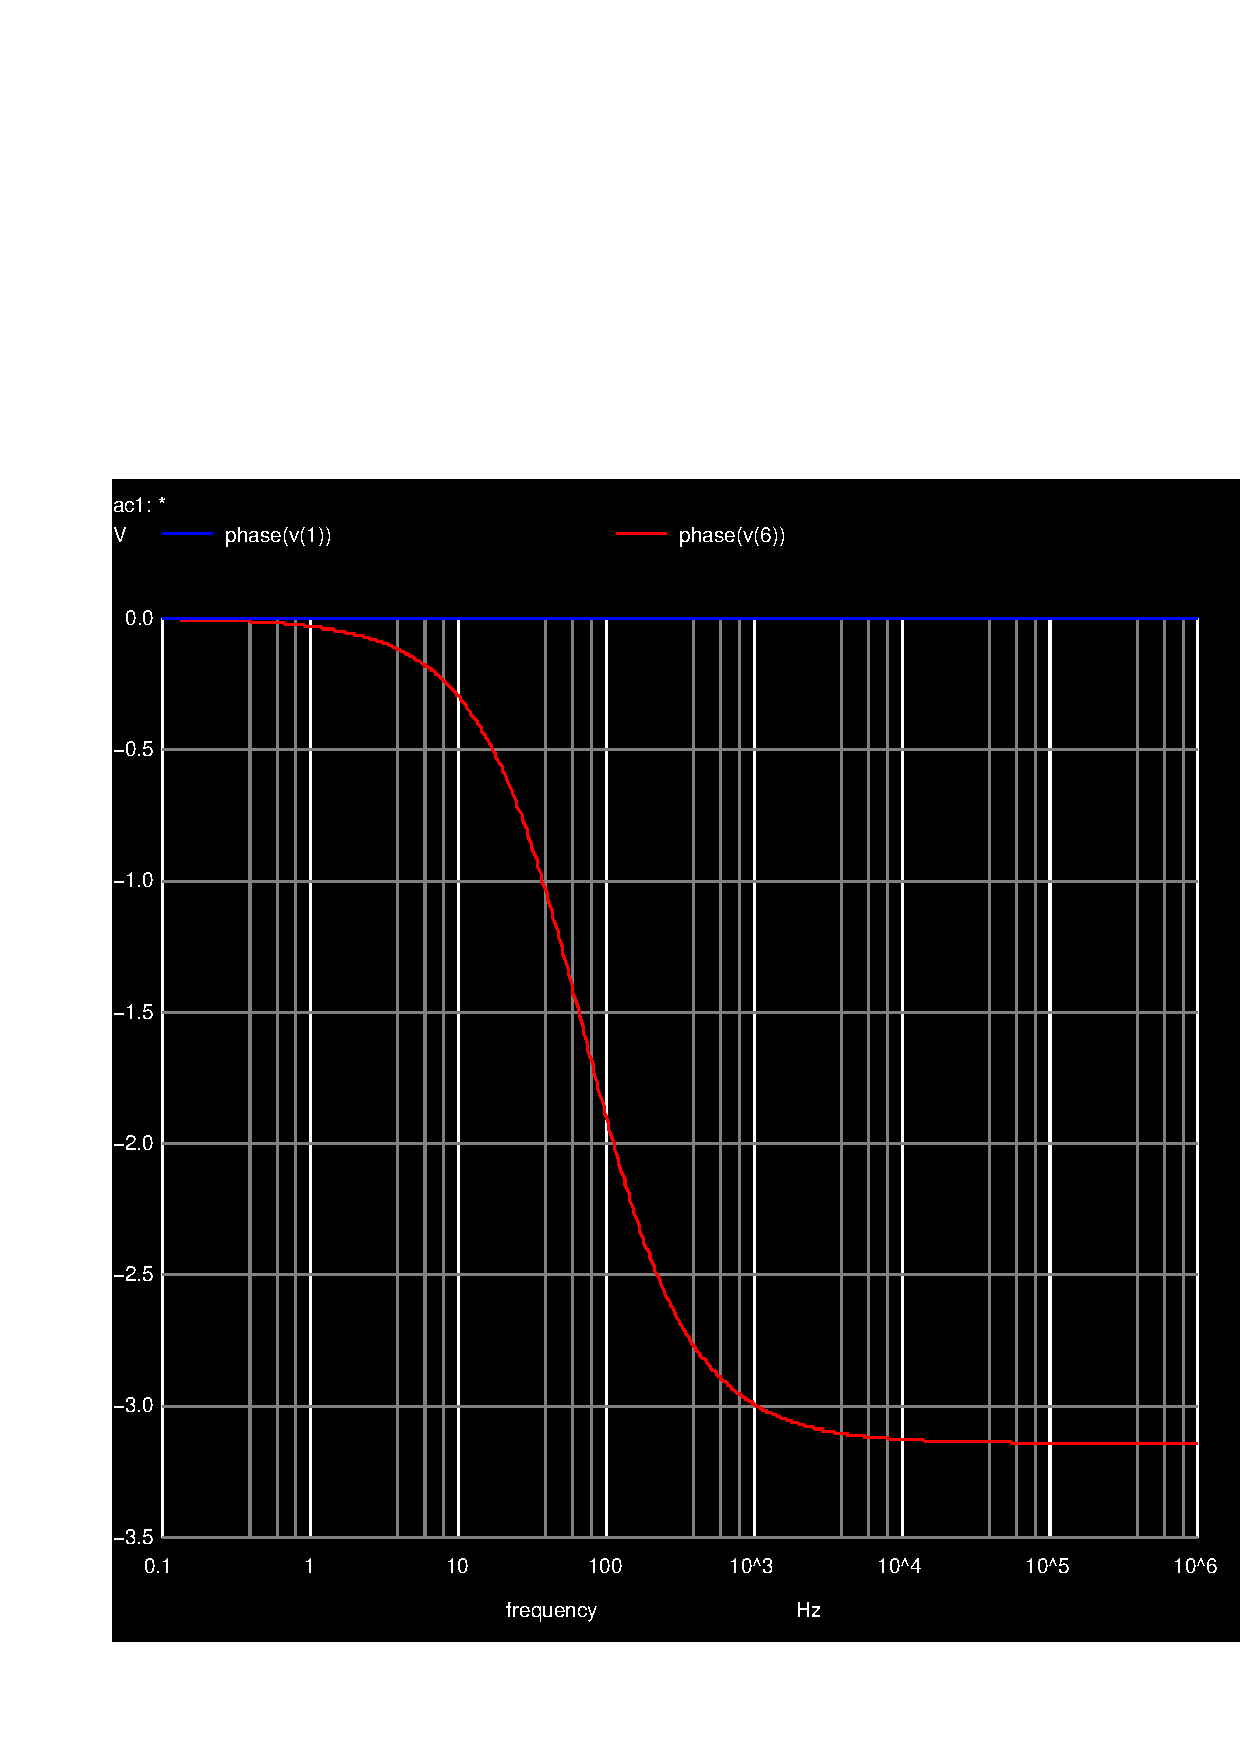
\includegraphics[width=0.4\linewidth]{acp.pdf}
%   \caption{Total solution for v(6) and $V_s$ in degrees}
%   \label{phase_spice}
% \end{figure}

% \begin{figure}[h] \centering
%   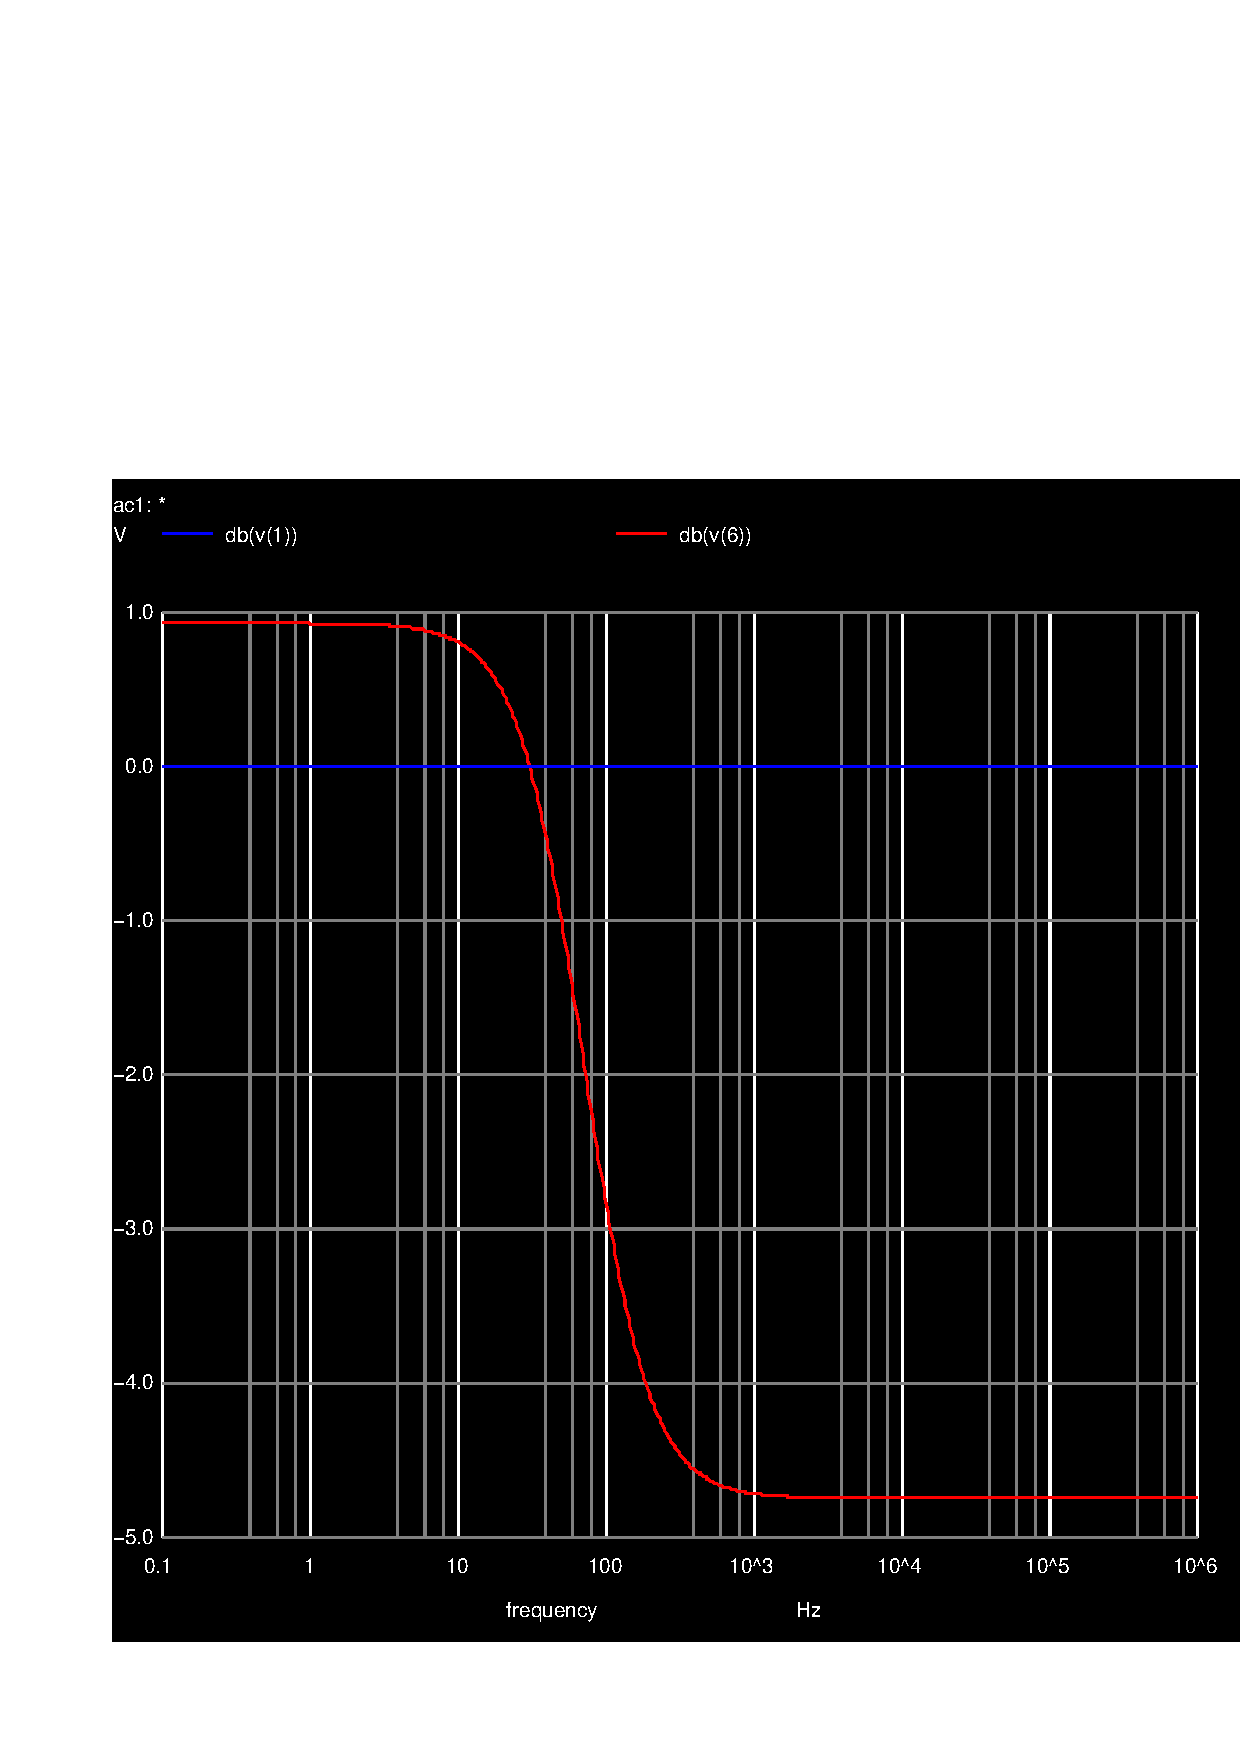
\includegraphics[width=0.4\linewidth]{acm.pdf}
%   \caption{Amplitude response for v(6) and $V_s$ in dB}
%   \label{amp_spice}
% \end{figure}


% Finally, with the goal of observing the low-pass filter nature 
% of the capacitor, we simulated the circuit for various frequencies of 
% $V_s$ (0.1Hz to 1MHz) and plotted the change in the phase (\ref{phase_spice}) 
% and in the amplitude (\ref{amp_spice}) of $V_s$ and $V_6$. Note that the 
% amplitude is expressed in dB's, justifying the negative values. Vs(f) is 0 as the ratio of it with itself is 1, therefore the logarithm is 0. As for V6(f), we can clearly observe the effect of the low-pass filter with the changes in output ratio for different frequencies.







%\lipsum[1-1]




